\documentclass{article}

%package setup
\usepackage{graphicx}
\usepackage{amsmath}
\usepackage{fancyhdr}
\usepackage[margin=1in]{geometry}
\usepackage{comment}
\usepackage{placeins}
\usepackage{parskip}
\usepackage{subcaption}
\usepackage{appendix}
\usepackage{soul}
\usepackage{comment}
\usepackage[hidelinks]{hyperref}
\usepackage{matlab-prettifier}
\usepackage{minted}
\usepackage{enumitem}
\usepackage{float}
\usepackage{textcomp, gensymb}

\pagestyle{fancy}
\fancyhf{} % Clear header/footer settings
\rhead{\thepage} % Page number on the right in the header
\lhead{ASE375 Lab Report 3} % Your lab report title on the left

\begin{document}

\begin{titlepage}
  \centering
  
\includegraphics[width=10cm]{ase-logo-formal.png}  % Adjust the width as needed
  \vspace{1cm}  % Add some vertical space
 
  \Large \textbf{ASE 375 Electromechanical Systems}\\
  \large \textbf{Section 14115}\\
  \vspace{0.5cm}
  \textbf{Monday: 3:00 - 6:00 pm}\\
 
  \vspace{1cm}
 
  \hrule
  \vspace{0.5cm}
 
  \Huge \textbf{Report 3:\\
  Measuring Displacement}\\
  \Huge \textbf{}\\
 
  \vspace{0.5cm}
  \hrule
 
  \vspace{1cm}
 
  \normalsize \textbf{Andrew Doty, Andres Suniaga, Dennis Hom}\\
  \normalsize \textbf{Due Date: 02/12/2024}
 
\end{titlepage}
\newpage

\tableofcontents
\thispagestyle{empty}
\newpage

\section{Introduction}
In this experiment we take a look at (1) Using a linear potentiometer to measure displacement of a small scale wing model with weights attached at different locations, (2) Determining the twist angle from these displacement measurements, and (3) Calculating the shear center, bending stiffness, and torsional stiffness of the wing model. 
\vspace(5mm)

This experiement attempts to accurately model measurements from the linear potentiometer in comparison to the ideal linear relationship from theoretical predictions. From these measurements we can then calculate the wing's shear center location and stiffness.  

\section{Equipment}
Devices used in this lab include:
\begin{itemize}

\item Digital Calipers: Used for measuring outer and inner dimensions of objects. In our case, digital calipers were used to measure the chord length of the small scale wing platofrm, the distance steps taken to calibrate the linear potentiometer, and the markings indicating chordwise locations for weight placement on the wing model.
\vspace{2.5mm}

\item Brass Slotted Weights with hanger: Used to induce bending on the wing model to acquire displacement measurements. Total 250 grams.
\vspace{2.5mm}

\item LP804 Series Miniature Linear Potentiometer: Device used to measure linear position and displacement from wing bending and twisting.
\vspace{2.5mm}

\item 'Rare Earth' Magnets: High strength magnets used for secure placement of linear potentiometer to the wing platform to acquire measurements without slippage.
\vspcae{2.5mm}

\item DAQ, NI-9215 Voltage Input Module, and LabVIEW: Data Acquisition System used to process data collected by digitizing the analog information into "bins" for a computer. NI-9215 used to measure the input voltage signals for the DAQ system. LabVIEW used to model voltages through the DAQ read from the linear potentiometer displacement.
\vspace{2.5mm}

\item Solderless Breadboard and Jumper Wires: Used to make connections from the linear potentiometer to power, ground, and signal for data collection.

\end{itemize}

\section{Procedure}
This section covers our procedure for this experiment broken into three parts:

\subsection{Calibration of Linear Potentiometer}
This first part contains our procedure for calibrating the linear potentiometer. Before beginning calibration, this part required connection setup of the linear potentiometer to the DAQ, NI-9215, and LabVIEW to collect and process data to model the input voltage measurements.

\begin{enumerate}
\item Ensure connection between the DAQ system (NI-9215) and the Linear Potentiometer is correct.
\vspace{2.5mm}

\item Take the potentiometer and place it on its side for better control of its displacement.
\vspace{2.5mm}

\item Using the digital calipers, measure from the base of the moving shaft on the linear potentiometer to the first displacement step $x_{1}$. We let the displacement step $\Delta x \approx 10\, mm$ for our calibration process. 
\vspace{2.5mm}

\item Repeat the displacement process for $i>=5$ times, i.e. the next step is $x_{2} \approx 20\, mm$. We let $i = 6$ with an additional final calibration measurement $\approx 20\, mm$ from the $x_{6}$ step to cover the full range of the $5V$ input voltage.

\end{enumeratre}

\subsection{Weight hanged at Chordwise locations}

\subsection{Weight hanged at Spanwise locations}

\section{Data Processing}
\subsection*{Variables}
\begin{enumerate}[label = \roman*.]
    \item
\end{enumerate}

\subsection*{Equations}
\begin{enumerate}[label = \Roman*.]
    \item 
\end{enumerate} 

Calibration:
\begin{table}[ht]
\centering
\begin{tabular}{|c|c|c|}
\hline
\textbf{X Position} & \textbf{Voltage Response} & \textbf{Standard Deviation} \\
\hline
$10 mm$ & $0.5706 V$ & 0.0007\\
\hline
$20.09 mm$ & $1.013 V$ & 0.00071 \\
\hline
$29.99 mm$ & $1.82 V$ & 0.00088 \\
\hline
$40.04 mm$ & $2.485 V$ & 0.0009\\
\hline
$50.01 mm$ & $3.023 V$ & 0.0008\\
\hline
$60.09 mm$ & $3.699 V$ & 0.00078\\
\hline
$80.06 mm$ & $4.996 V$ & 0.0004\\
\hline
\end{tabular}
\caption{Table of X Position and Voltage Response}
\label{tab:position_voltage}
\end{table}

C = 100.8 mm

\begin{table}[ht]
\centering
\begin{tabular}{|c|c|c|}
\hline
\textbf{X Position} & \textbf{Voltage Response} & \textbf{Standard Deviation} \\
\hline
$0 mm$ & $2.146 V$ & 0.00093 \\
\hline
$10 mm$ & $2.164 V$ & 0.00099\\
\hline
$20 mm$ & $2.184 V$ & 0.00095\\
\hline
$30 mm$ & $2.200 V$ & 0.0010 \\
\hline
$40 mm$ & $2.227 V$ & 0.00093 \\
\hline
$50 mm$ & $2.256 V$ & 0.0010 \\
\hline
$60 mm$ & $2.279 V$ & 0.00099 \\
\hline
$70 mm$ & $2.306 V$ & 0.00098 \\
\hline
$80 mm$ & $2.334 V$ & 0.00097\\
\hline
$90 mm$ & $2.363 V$ & 0.00100\\
\hline
$100 mm$ & $2.384 V$ & 0.00096\\
\hline
\end{tabular}
\caption{Table of X Position, Voltage Response, and Standard Deviation Trailing Edge}
\label{tab:position_voltage_stddev}
\end{table}

Calipers go to 0.5 mm in least count
250g weight



\begin{table}[ht]
\centering
\begin{tabular}{|c|c|c|}
\hline
\textbf{X Position} & \textbf{Voltage Response} & \textbf{Standard Deviation} \\
\hline
$0 mm$ & $1.979 V$ & 0.00096\\
\hline
$10 mm$ & $1.988 V$ & 0.00096 \\
\hline
$20 mm$ & $1.988 V$ & 0.00096 \\
\hline
$30 mm$ & $1.985 V$ & 0.00095 \\
\hline
$40 mm$ & $1.993 V$ & 0.00096 \\
\hline
$50 mm$ & $1.997 V$ & 0.00100 \\
\hline
$60 mm$ & $1.990 V$ & 0.00099 \\
\hline
$70 mm$ & $2.004 V$ & 0.00097 \\
\hline
$80 mm$ & $2.005 V$ & 0.00099 \\
\hline
$90 mm$ & $2.014 V$ & 0.00100 \\
\hline
$100 mm$ & $2.014 V$ & 0.00098 \\
\hline
\end{tabular}
\caption{Table of X Position, Voltage Response, and Standard Deviation Leading Edge}
\label{tab:position_voltage_stddev2}
\end{table}

\subsection{Part 2}

\begin{table}[ht]
\centering
\begin{tabular}{|c|c|c|c|}
\hline
\textbf{Potential Position} & \textbf{Weight Position} & \textbf{Volts} & \textbf{Std} \\
\hline
$5$ & $6$ & $2.501 V$ & 0.00093 \\
\hline
$2$ & $6$ & $2.234 V$ & 0.00099 \\
\hline
$4$ & $6$ & $2.809 V$ & 0.00095 \\
\hline
$1$ & $6$ & $2.471 V$ & 0.00090 \\
\hline
$3$ & $6$ & $1.988 V$ & 0.00097 \\
\hline
$6$ & $6$ & $2.102 V$ & 0.00100 \\
\hline
$5$ & $5$ & $2.599 V$ & 0.00100 \\
\hline
$2$ & $5$ & $2.312 V$ & 0.00096 \\
\hline
$4$ & $5$ & $2.873 V$ & 0.00096 \\
\hline
$1$ & $5$ & $2.505 V$ & 0.00090 \\
\hline
$4$ & $4$ & $2.904 V$ & 0.00099 \\
\hline
$1$ & $4$ & $2.564 V$ & 0.00098 \\
\hline
\end{tabular}
\caption{Table of Potential Position, Weight Position, Volts, and Std}
\label{tab:position_weight_volts_std}
\end{table}



\section{Results and Analysis}

\section{Conclusion}

\newpage
\thispagestyle{empty}  % Clear header/footer
\begin{center}
	\vspace*{\fill}
	{\Huge Appendices}
	\vspace*{\fill}
\end{center}

% Start appendices
\newpage
\begin{appendices}
\pagestyle{fancy}
\renewcommand{\thefigure}{A\arabic{figure}}
\setcounter{figure}{0}

\section*{Appendix: t-Distribution Tables}
\hypertarget{1}{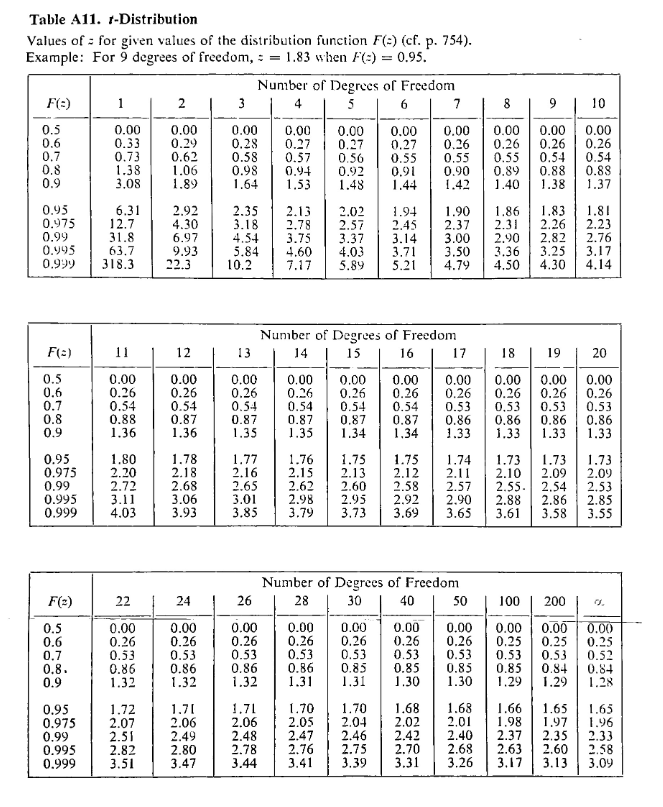
\includegraphics[width=0.95\textwidth]{t_distribution_Table_lecture3.png}}
\end{appendices}

\end{document}
